\section{Controlled Toy Example}
\label{sec: toy example}
Generally, the two effects interact during end-to-end co-training and jointly influence the learning dynamics. To disentangle and understand their individual contributions to co-training, we designed a pilot toy experiment.
In this simplified setting, we seek to learn a policy model $\pi_\theta$ with a pre-trained feature encoder that defines the input distribution $p(x)$, where each input dimension corresponds to a principal direction in the latent space.
We adopt a 4-layer Multi-Layer Perceptron (MLP) as the diffusion model architecture.
% This assumption holds reasonably well, since the model we use is a shallow 4-layer Multi-Layer Perceptron (MLP).

\textbf{Experiment design.}
The policy model $\pi_\theta$ is co-trained to learn the mapping $\pi(y|x):\mathbb{R}^3 \rightarrow \mathbb{R}^2$.
We manually define two manifolds, $\mathcal{M}_S$ and $ \mathcal{M}_T$, with different distributions, corresponding to the intrinsic data distributions of the source and target domains, respectively.
Then, we sample paired data points from these two manifolds $D_S=\{(x_i, y_i)\}^{N_S}\sim\mathcal{M}_S$ and $D_T=\{(x_i, y_i)\}^{N_T}\sim\mathcal{M}_T$, where $N_S \gg N_T$ and $D_T$ is sampled partially as shown in Fig.~\ref{fig:toy-example}.
This design simulates the common case in which target domain data is usually sparser, limited, and less diverse than source data.
We align the two manifolds along two principal directions but vary the distance between them along the remaining one to create different representation alignment scenarios.
The results are shown in Fig.~\ref{fig:toy-example}.
% We quantitatively measure the in-distribution and out-of-distribution prediction error since we know the ground-truth mapping.

\textbf{Finding 1: The toy model behavior aligns with our theoretical analysis.}
 As expected, under three different representation scenarios described in Sec.~\ref{sec: condition representation}, the co-trained model exhibits distinct behaviors: 
 1) In disjoint, the prediction remains close to that of the model trained solely on target-domain data, where the model can easily distinguish between two domains but fails to transfer knowledge, i.e., the learned mapping, from the source domain. Due to the limited amount of data, the model tends to memorize each data point~\cite{he2025demystifying}, failing to interpolate within the training distribution and extrapolate beyond it.
 2) In structured alignment, this setting represents a sweet spot, where the model achieves a balance between representation alignment and domain discernibility. As a result, the output distribution is reconstructed with high fidelity.
 3) In overlapping, the model predictions become randomly distributed between the source and target domains. Here, the model cannot effectively distinguish between the two domains and instead treats them as identical, preventing meaningful adaptation of transferred knowledge.
 On the other hand, the data mixing ratio $w$ exerts an independent but secondary influence on this capability via importance reweighting, as discussed in Sec.~\ref{sec: balanced mixing ratio}.
Specifically, it adjusts the relative amplitude of transferred knowledge $s^*_s$ and target-domain adaptation $s^*_t$.
As illustrated by the horizontal comparison in Fig.~\ref{fig:toy-example}, when $w$ is relatively small (e.g., the second column from the left), the output becomes noisier due to the increased contribution of source-domain data during the early denoising steps.
% \begin{itemize}[leftmargin=*]
%     \item \textbf{Disjoint}. The model prediction remains close to that of the model trained solely on target-domain data. In this case, the model can easily distinguish between the two domains but fails to transfer knowledge — i.e., the learned mapping — from the source domain. Owing to the limited amount of data, the model tends to memorize individual data points~\cite{he2025demystifying}, rather than learning a smooth function that interpolates within the training distribution or extrapolates beyond it.
%     \item \textbf{Structured alignment}. This setting represents a sweet spot, where the model achieves a balance between representation alignment and domain discernibility. As a result, the output distribution is reconstructed with high fidelity.
%     \item \textbf{Overlapping}. The model predictions become randomly distributed between the source and target domains. Here, the model cannot effectively distinguish between the two domains and instead treats them as identical, preventing meaningful adaptation of transferred knowledge.
% \end{itemize}

In addition, we observe an intriguing phenomenon: with appropriate co-training settings, the model can reasonably make predictions in the out-of-distribution (OOD) region, indicating OOD generalization capability. Notably, this capability does not arise from simply copying knowledge from the source domain; rather, it emerges from preserving the distribution shift in the learned representations, which is crucial for accurate OOD prediction.

\textbf{Finding 2: Structured representation alignment is a dominant driver of strong model performance.}
Since we have the ground-truth mapping, we provide a quantitative measure using $L2$ loss in Fig.~\ref{fig: sweep toy}.
The overall importance reweighting effect is constrained by the underlying representation alignment. That is, changing the mixing ratio alone cannot compensate for poorly aligned representations, nor can it induce OOD generalization in the absence of sufficient alignment, \textit{e.g.}, the red and blue curves where the mixing ratio nearly has no effect on the final performance.
Based on this, we conduct an ANOVA-style variance decomposition analysis~\cite{fisher1971design} on these two factors. 
We find that changes in structured representation alignment explain around $50\%$ of the loss variance, while the importance reweighting effect of the mixing ratio accounts for only $20\%$.
In this sense, structured representation alignment is the primary determinant of model behavior, while $w$ serves as a modulation factor that fine-tunes the balance between source and target domain knowledge. 

% More detailed sweeping results are available in Appendix.~\ref{appdx: detailed toy measure}.

% Since the ground-truth mapping is known in this toy setting, we quantify the prediction error to explicitly characterize the effects of these two factors.
% The details of the quantitative  can be found in the Appendix.\textcolor{red}{add appendix ref}

\begin{figure}[htbp]
    \centering
    \captionsetup{font={small}}
    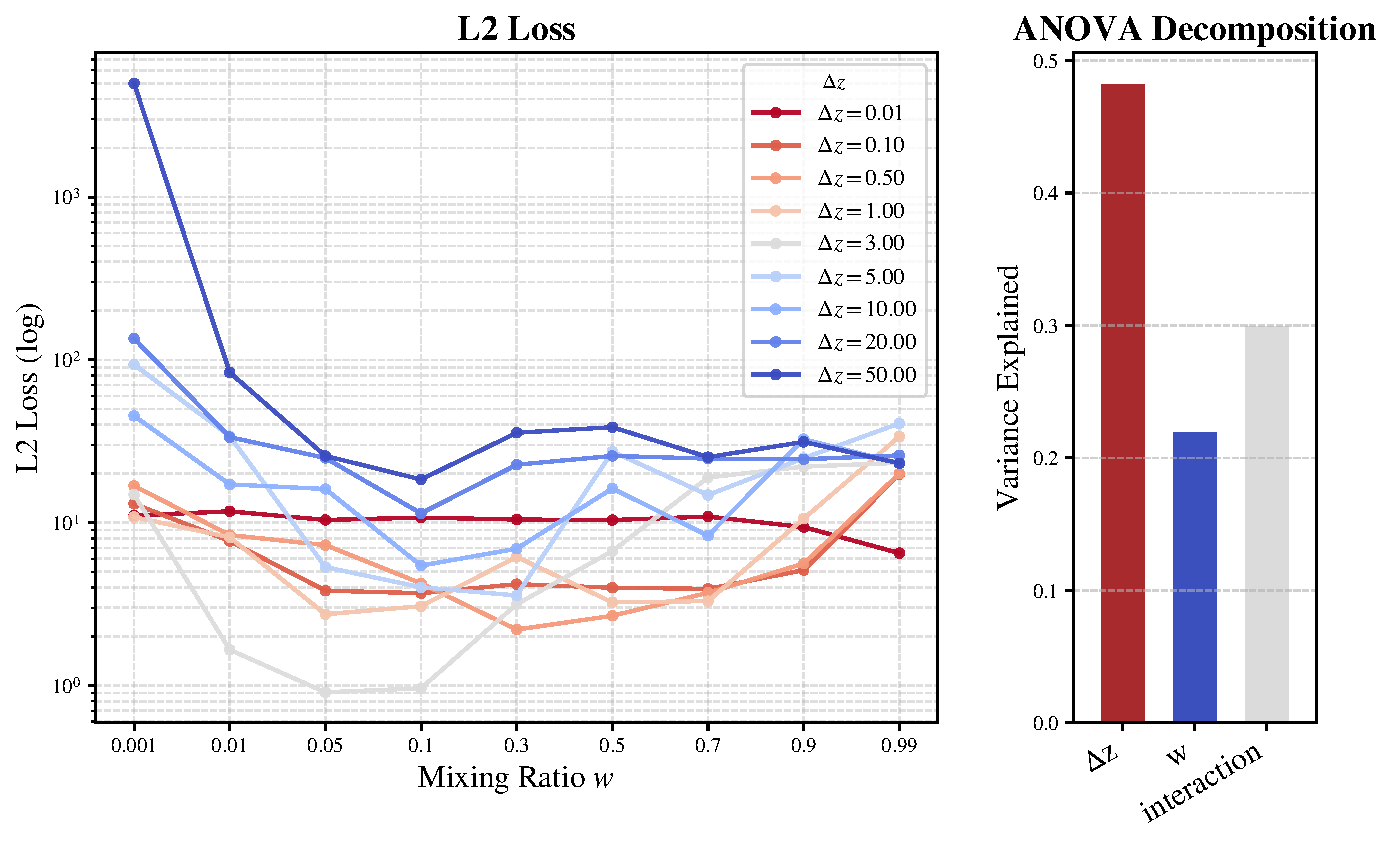
\includegraphics[width=\linewidth]{asset/quantitative_toy_example.pdf}
    % \vspace{-10pt}
    \caption{\textbf{L2 loss with sweeping mixing ratio and delta $z$ distance, and ANOVA variance decomposition.} When representations overlap (red line) or are disjoint (blue line), co-trained models are insensitive to mixing ratios. The importance reweighting effect (blue bar) can only explain $20\%$ of the performance variance.}
    \label{fig: sweep toy}
    \vspace{-10pt}
\end{figure}

By drawing an analogy from the toy example to sim-and-real co-training, we hypothesize a similar underlying mechanism: structured representation alignment enables effective knowledge transfer from simulation, while maintaining sufficient domain discernibility to adapt actions to the real world. A key question, however, is whether this mechanism can be empirically observed in practical sim-and-real settings, rather than remaining a purely conceptual intuition.

Moreover, \textit{Finding 2} raises a deeper question: can structured representation alignment emerge in end-to-end co-training, given that the data mixing ratio 
$w$ is the only explicit control variable? To answer these questions, we conduct extensive experiments on real-world robotic manipulation tasks.




\section{Sim-and-Real Co-Training for Manipulation}
\label{sec: manipulation experiments}

To find out more empirical evidence to validate our hypothesis in robot manipulation, in particular, sim-and-real co-training, we design a set of sim-and-sim and sim-and-real co-training experiments on manipulation tasks (Fig.~\ref{fig: task vis}).
The sim-and-sim experiments are designed to explicitly control the domain gaps between source and target domains to ensure our observations are consistent across different domain gaps.
Across all experiments, we adopt a transformer-based diffusion model~\cite{chi2025diffusion} with ResNet18~\cite{he2016deep} as the vision backbone and train end-to-end.

% The results show that 
% (1) \textit{representation alignment correlates with model performance} (Sec.\ref{sec:representation alignment}) - it's beneficial to strength alignment,
% (2) but at the same time, \textit{it is also necessary for models to distinguish representations from different domains} (Sec.\ref{sec: discernibility}).




% \begin{table}[t]
% \centering
% \small
% \begin{tabular}{lccc}
% \toprule
%  & \textbf{Visual} & \textbf{Env-Physics} & \textbf{Embodiment} \\
% \midrule
% vis-only   & \checkmark &              &              \\
% phys-only   &             & \checkmark   &              \\
% vis-phys  & \checkmark & \checkmark   &              \\
% vis-phys-robot     & \checkmark & \checkmark   & \checkmark   \\
% \midrule
% sim--real  & \checkmark & \checkmark   &              \\
% cross-embodiment      & \checkmark &              & \checkmark   \\
% \bottomrule
% \end{tabular}
% \caption{\textbf{Domain shift decomposition}. We create 4 sim-and-sim settings to cover all of them.}
% \label{tab: gap decomposition}
% \end{table}
\textbf{Task suites.}
We choose three manipulation tasks from robosuite~\cite{zhu2020robosuite}: \texttt{NutAssembly}, \texttt{MugHang}, and \texttt{MugCleanup}.
\texttt{NutAssembly} and \texttt{MugHang} require more precise control than common pick-and-place tasks, as it includes dense object interactions. And there are more rotation motions in the actions of \texttt{MugHang} demonstrations.
In addition, the model needs relatively long-horizon reasoning and execution to succeed in \texttt{MugCleanup}.
These tasks represent many key challenges in robot manipulation.


\textbf{Environment setup.}
For sim-and-real experiments, following the recipe in~\citet{maddukuri2025sim}, we calibrate the camera pose and intrinsics to minimize camera alignment differences between simulation and the real world.
% We roughly align the object placement regions, but there are still notable discrepancies, including controller parameters and physical parameters, etc.
For sim-and-sim experiments, we utilize the same \textit{source-sim} environments and create a second \textit{target-sim} environment with domain gaps.

\begin{figure*}[tbp]
\centering
    \includegraphics[width=0.9\linewidth]{asset/task_vis.pdf}
    \caption{\textbf{Visualizations of the designed sim-and-sim and sim-and-real tasks.} In the \textit{physics-only} setting, we vary the physical parameters of objects, including mass, friction, and size, while keeping the appearance similar. Across all target environments, we tune the robot controller configurations to match those in the real world.}
    \label{fig: task vis}
    \vspace{-10pt}
\end{figure*}

\textbf{Domain gaps categorization.} Simulation and the real-world data contain domain shifts from various aspects.
To identify the different effects of co-training across them, we decompose the gaps along two dimensions — visual appearance and environment physics. We manually introduce these gaps and construct three sim-and-sim co-training settings, \textit{i.e.}, \textit{visual-only}, \textit{physics-only} and \textit{visual-physics}.


% For the sim-and-sim experiments in this section, we conduct experiments on all of them to understand different domain gaps and ensure our observations are consistent.


\textbf{Data preparation.}
For the target domains, we collect 50 human demonstrations for each task.
For the source domains, we use MimicGen~\cite{mandlekar2023mimicgen} to further synthesize $\sim$3000 trajectories based on 50 human demonstrations.
Following ~\citet{wei2025empirical}, we define $w_n=\frac{|D_r|}{|D_r|+|D_s|}$ as the natural mixing ratio, where $|D_r|$ and $|D_s|$ are the sizes of real-world and simulation datasets, respectively. This is equivalent to concatenating the sim and real datasets.
For experiments in this section, we co-train policies by sweeping a set of mixing ratios $w\in \{ 0, 0.005, w_n=0.016, 0.1, 0.3, 0.5, 0.8, 1\}$.

\subsection{Observations on Representation Alignment}
\label{sec: representation alignment}

\textbf{Representation alignment can be learned \textit{implicitly} in end-to-end co-training.}
Our experiments began with visualizing the latent embeddings of simulation and real-world observation features across different layers using UMAP~\cite{mcinnes2018umap} at different mixing ratios.
Specifically, we look into the features after the vision stem and the final-layer output embeddings of encoder trunk $f_\phi$, which include other modality information such as proprioception and language.
What is surprising is that, in a certain range of mixing ratios, visual features exhibit local geometry alignment sharing very similar geometric structures, while the observation features show representation alignment in global space, as shown in Fig.~\ref{fig:feature vis}.
This can inform us about how the representation alignment evolves through the networks.
We further quantify the local and global representation alignment using the Gromov-Wasserstein distance~\cite{memoli2011gromov} and Wasserstein distance~\cite{ruschendorf1985wasserstein}, respectively.
By varying the data mixing ratio, we observe a clear correlation: smaller distances between real and simulation features correspond to more similar latent geometries and stronger alignment as shown in Fig.~\ref{fig:feature vis} (Full visualizations are available in Appendix~\ref{appdx: more feature vis}).
This trend holds consistently across both sim-to-real and sim-to-sim experiments. These results suggest that co-training remains sensitive to the data mixing ratio $w$ because adjusting it simultaneously and substantially alters primary intrinsic effect—representation alignment itself. In other words, the mixing ratio does not merely re-weight source and target data contributions, but also implicitly reshapes the learned representation space. Similar phenomena have also been observed in \citet{kareer2025emergence}, where the alignment emerges from scaling pre-training data.
% Another interesting thing is that we also visualize the vision encoder features, which have not been further processed with proprioception and language embedding. 
% For features in the balanced mixing ratio range, vision encoder features exhibit local geometry alignment with very similar structures while final-layer features show alignment in global space, as shown in Fig.~\ref{fig:feature vis}.
% We hypothesize that preserving a similar geometric structure is the prerequisite for structured representation alignment.
% Specifically, we take the final layer output embeddings of the observation encoder $f_\phi$, then standardize 

\begin{figure*}[t]
\centering
    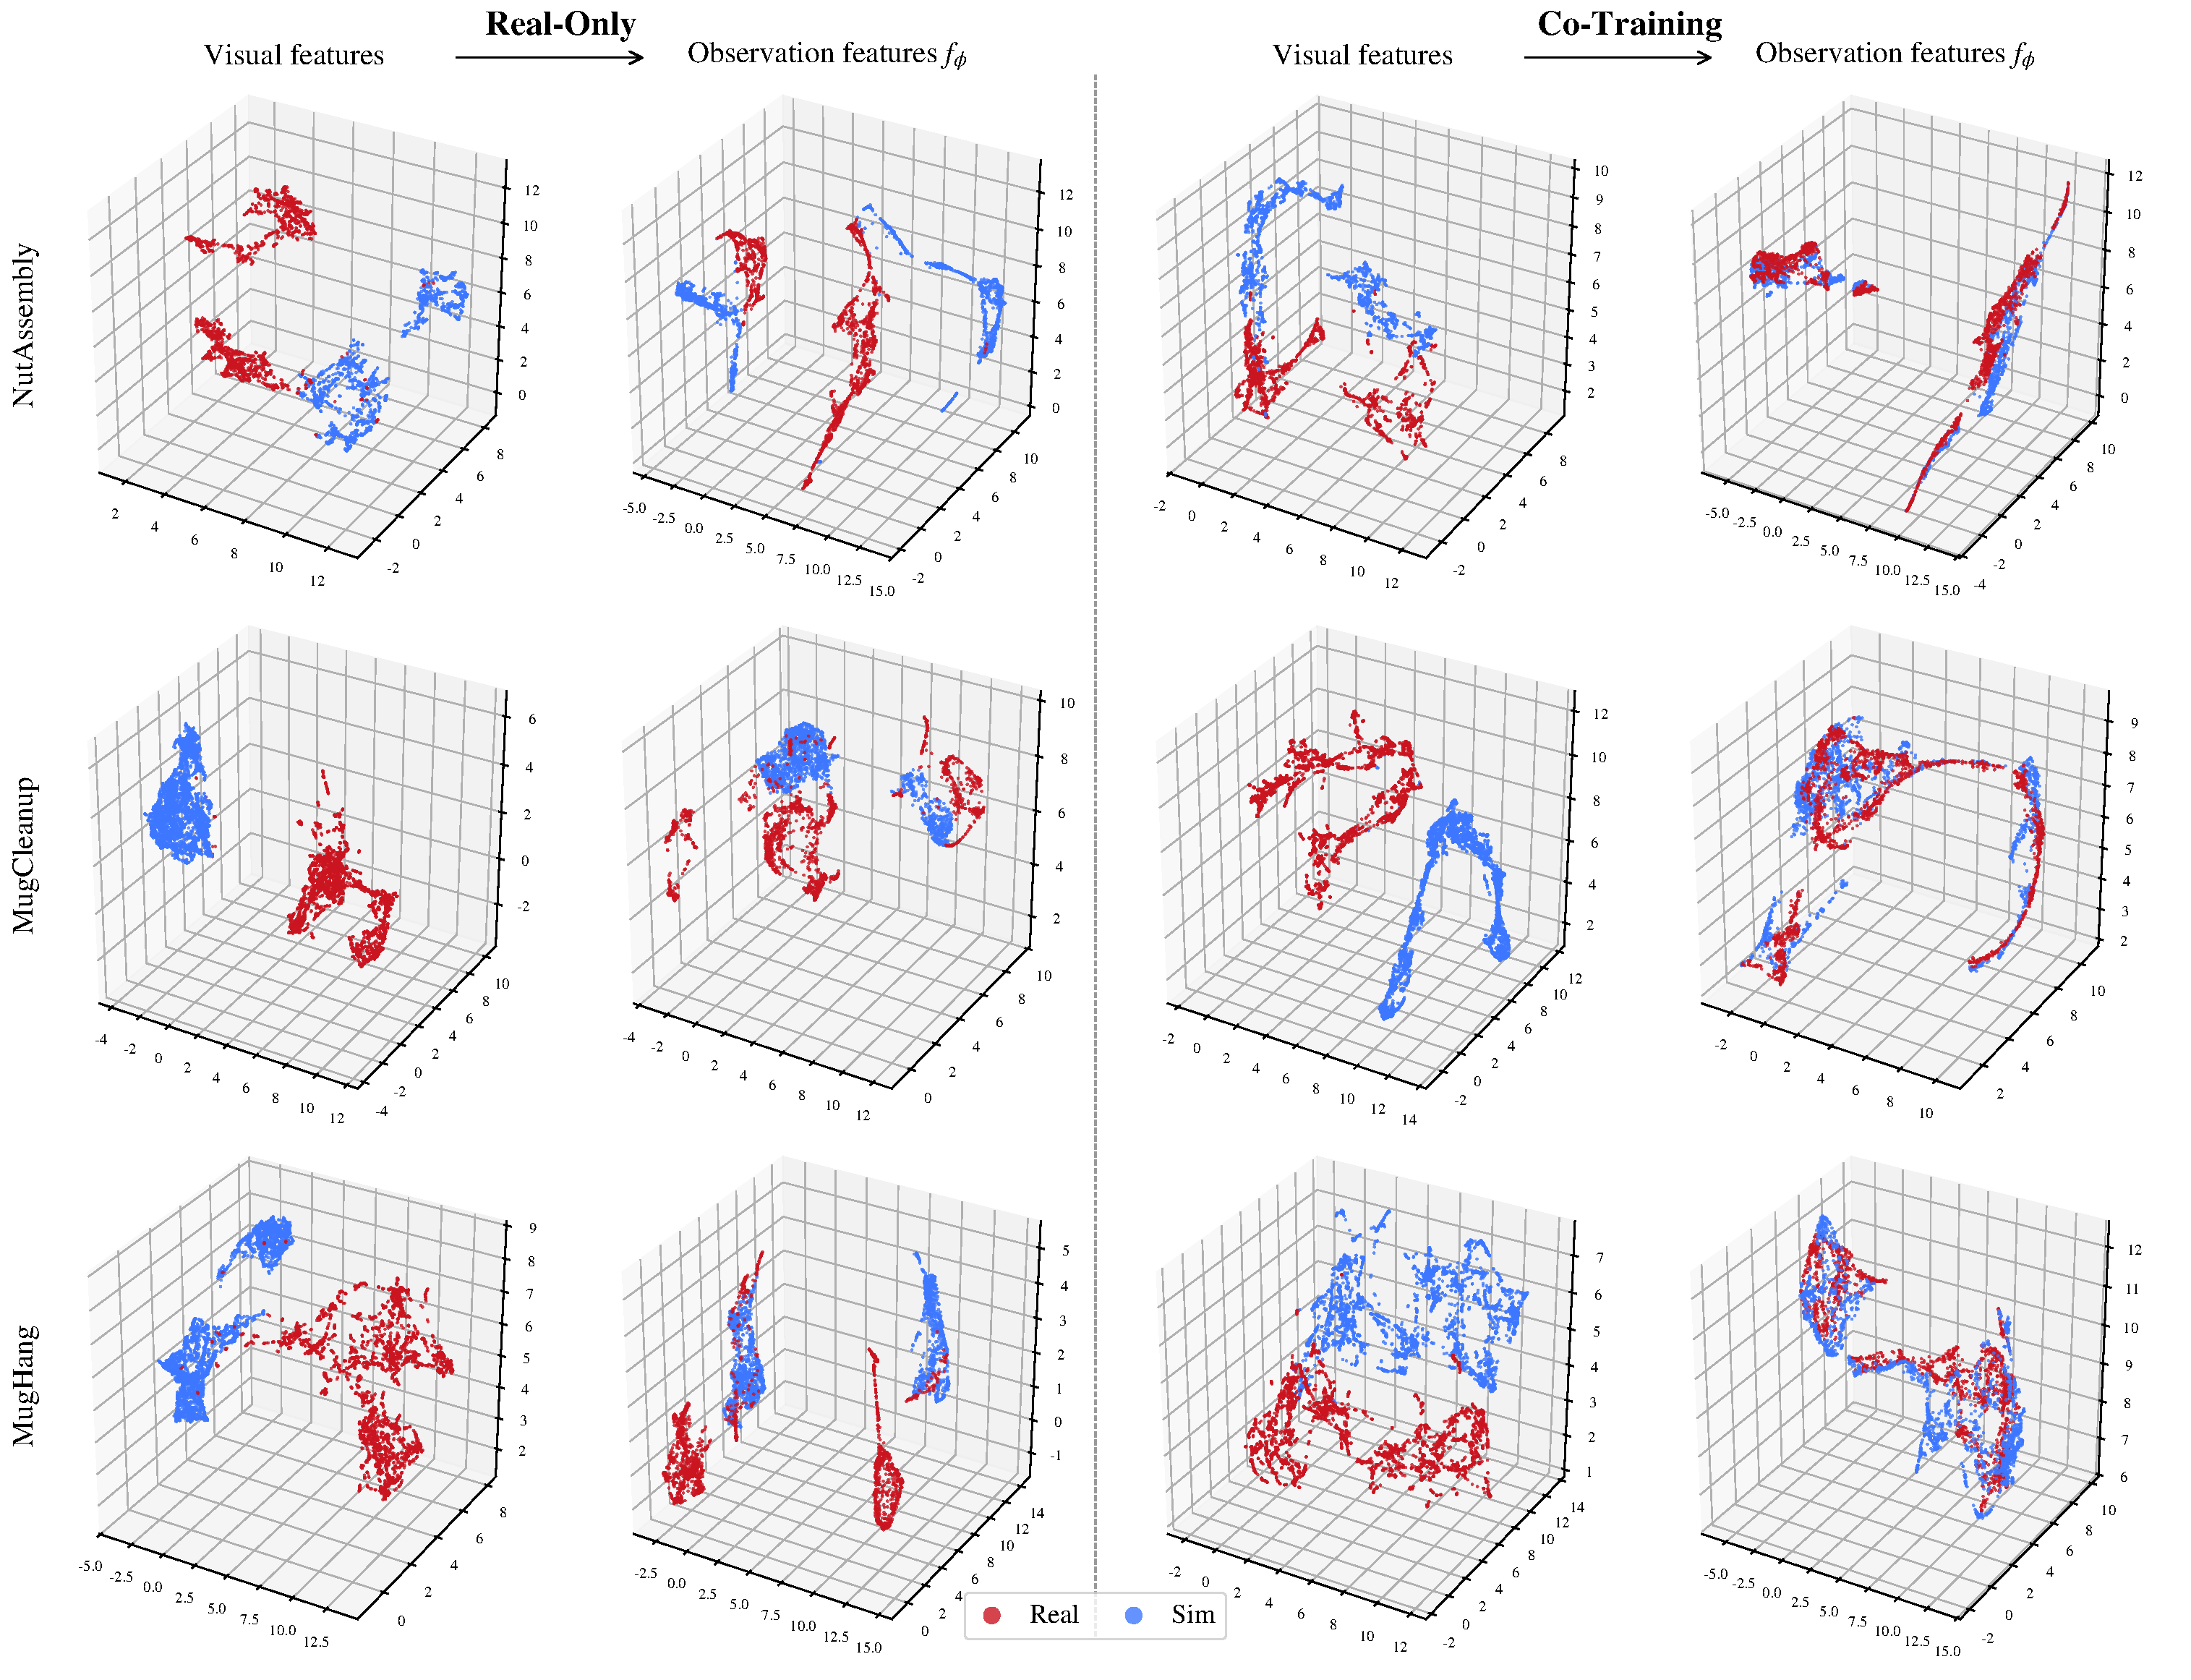
\includegraphics[width=0.95\linewidth]{asset/feat_vis_test.pdf}
    \caption{\textbf{UMAP visualization of latent features.} We visualize the features after the vision stem and after the encoder trunk $f_\phi$. Red and blue dots represent the real and simulation features, respectively. We show the results for a specific mixing ratio in this figure. More details and results are provided in the Appendix~\ref {appdx: more feature vis}.}
    \label{fig:feature vis}
    \vspace{-5pt}
\end{figure*}

\begin{figure*}[htbp]
\centering
    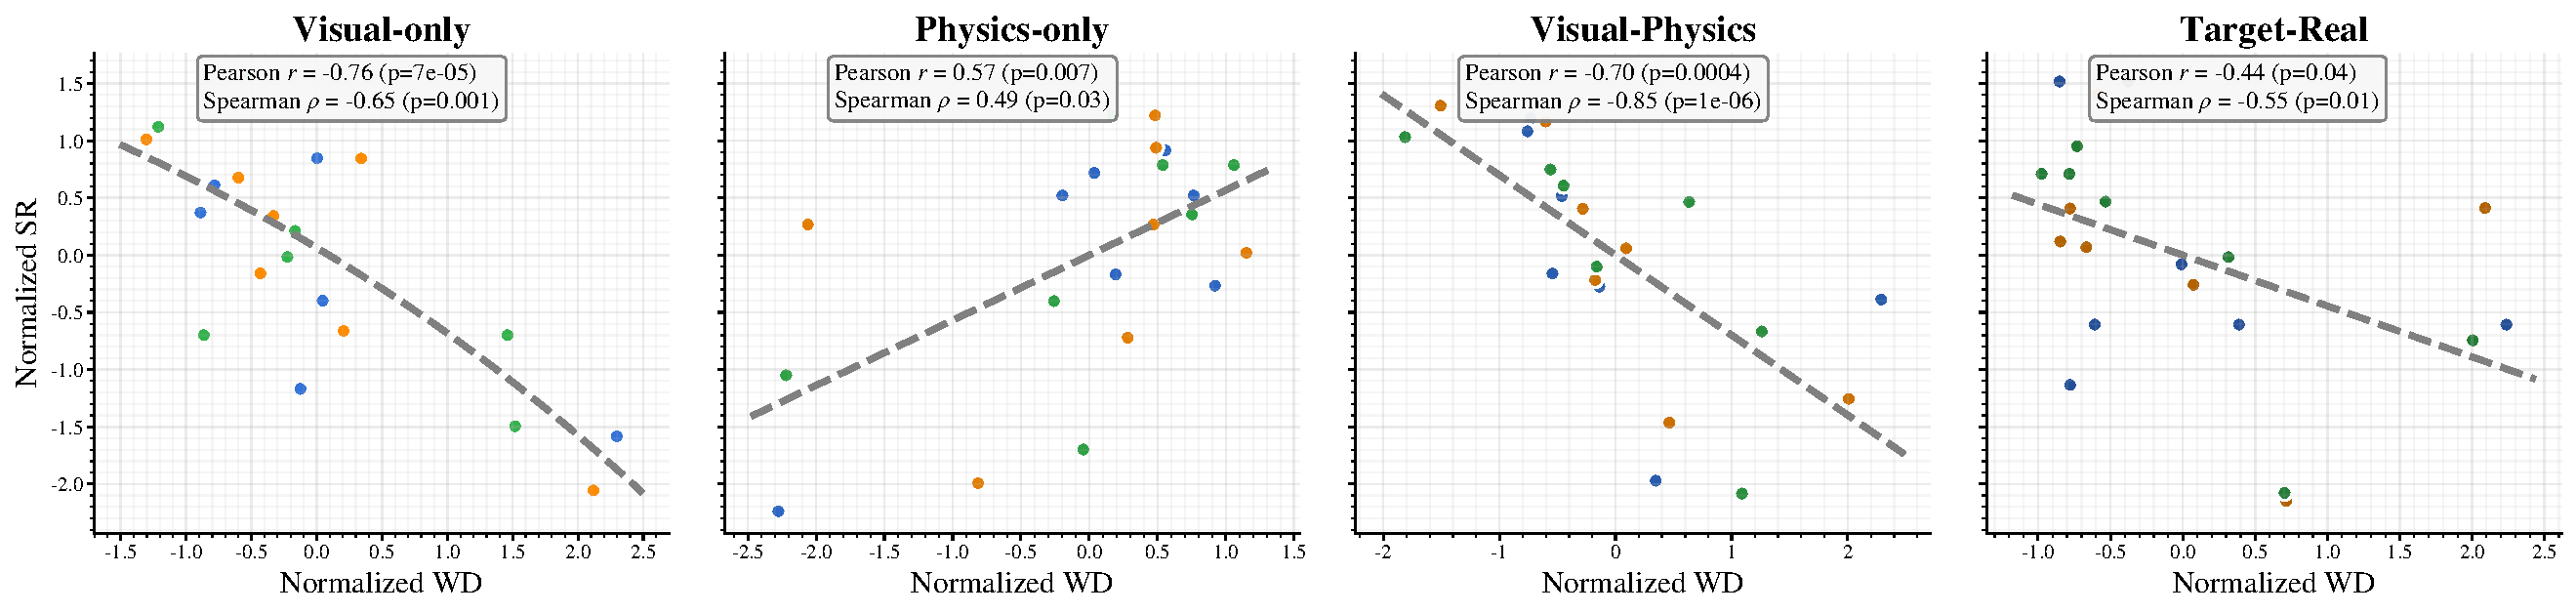
\includegraphics[width=0.95\linewidth]{asset/sim2sim_correlation.pdf}
    \caption{\textbf{Correlation between representation alignment and success rate.} We group the results of different tasks in each setting and compute the Spearman and Pearson correlation coefficients after normalization. Blue, yellow, and green-series dots represent the same task in Fig.~\ref{fig: success rate}. Gray dash line indicates the fitted curve.}
    \label{fig:correlation}
\end{figure*}

\begin{figure*}[tbp]
\centering
    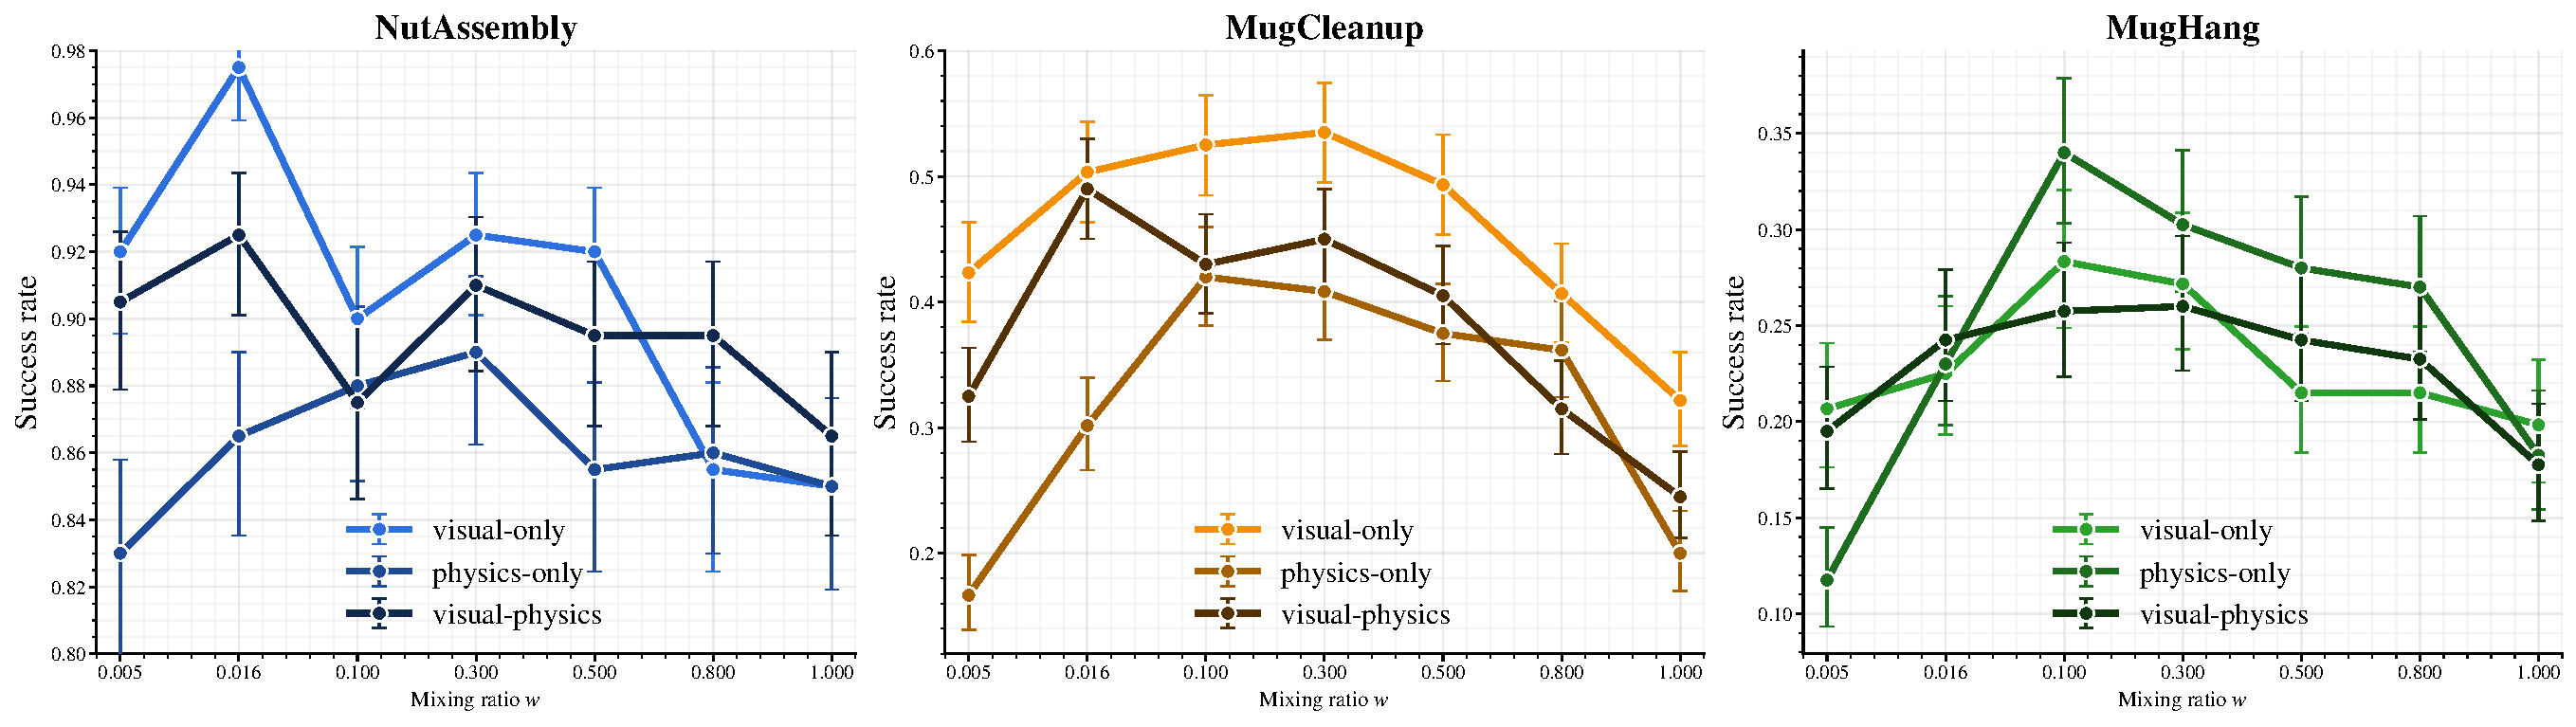
\includegraphics[width=0.95\linewidth]{asset/sim2sim_gap_success_rates_with_ci.pdf}
    \caption{\textbf{Success rate of sim-and-sim co-training with different domain gaps.} Each data point is computed over three policy checkpoints, and each checkpoint is evaluated for 200 trials.
    The best performance is consistently achieved in the range of $(0.016, 0.3)$.}
    % We can find that as the domain gaps increase, the model performance usually drops, \textit{e.g.} from visual-only to visual-physics.}
    \label{fig: success rate}
\end{figure*}


\textbf{Representation alignment \textit{positively correlates} with model performance.}
% We use the success rate as a measure of model performance.
% For each checkpoint of the sim-and-sim co-trained policy, we evaluate the policy over 200 simulation episodes and report the mean success rate.
% For each sim-and-real co-trained policy, we evaluate performance over 15 random trials.
We compute the correlation between the log-transformed Wasserstein distance obtained above and the corresponding success rate across different settings.
For each checkpoint, we evaluate the policy over 200 trials (sim) and 30 trials (real) for computing the mean success rate.
We report both Pearson’s correlation coefficient, which captures linear associations, and Spearman’s rank correlation coefficient, which is robust to non-linear but monotonic relationships.
As shown in Fig.~\ref{fig:correlation}, in all settings except the physics-only condition in sim-and-sim co-training, both Pearson and Spearman correlation coefficients fall in the range of $0.6\sim0.8$, with p-values $<0.04$. These results indicate a moderate-to-strong positive association between representation alignment and model performance. In some cases, one of the correlation coefficients (Pearson or Spearman) is lower (e.g., 
$\sim0.4$), suggesting that the relationship may be non-linear or only partially monotonic rather than strictly linear. Importantly, this overall pattern is consistently observed across all three tasks.


\textbf{Suppressing representation alignment results in performance degradation.}
To further verify the causal effect of representation alignment, we conduct a minimal ablation that explicitly encourages representation separation in \textit{vis-phys} sim-and-sim setting.
Inspired by adversarial domain adaptation~\cite{tzeng2017adversarial}, we keep the domain classifier operating on the learned representation, but intentionally remove the gradient reversal layer, thereby promoting domain-discriminative features instead of domain-invariant ones.
The performance across 3 tasks drops consistently.

\begin{table}[hb]
\centering
\vspace{-0.2em}
% \vspace{-1em}
\resizebox{\linewidth}{!}{
\begin{tabular}{c|c|c|c|c}
    \toprule
                            &NutAssembly    &MugCleanup    &MugHang    &Avg \\
    \midrule
     co-training&   0.85    &     0.44  &    0.27  &   0.52   \\
    % \cmidrule{2-6}
    \midrule
     +discrimination  &   0.79  &    0.415  &   0.215   &   0.47   \\
    \bottomrule
\end{tabular}
}
\caption{\textbf{Performance degrades after adding penalty for representation alignment.} The experiments are run with $w=0.1$.}
% % \vspace{+.5em}
% % \captionsetup{font={tiny}}
% \label{tab:quantitative comparison}

\end{table}



\subsection{Observations on Domain Discernibility}
\label{sec:discernibility}
% However, as we analyze and observe in Sec.~\ref{sec: condition representation} and Sec.~\ref{sec: toy example}, this section shows that \textit{domain discernibility is necessary for successful co-training}.

\textbf{Although representations align in low-dimensional space, they are easily discernible by shallow neural networks.}
We perform a simple linear probing study by training a 2-layer MLP for binary-domain classification on the encoder trunk's output embeddings.
Surprisingly, even if the representations seem to be aligned well in low-dimensional space, a simple MLP can easily achieve $\sim100\%$ success rate on validation sets in all settings.
This suggests that representations are in the partially aligned scenario, and co-training policies do retain the domain-specific information.

\textbf{Discernibility is \textit{indispensable} for actions to adapt to the target domain.}
We report the success rate of each task in each setting in Fig.~\ref{fig: success rate}.
We can find that in the four sim-and-sim settings, the success rate of the \textit{physics-only} policy is even lower than the \textit{vis-phys} policy on the task of \texttt{NutAssembly} and \texttt{MugCleanup}.
As we largely change the object's physical parameters while keeping its visual appearance similar, it is harder for co-trained policies to distinguish between the two environments.
Interestingly, from Fig.~\ref{fig:correlation}, we observe that the correlation between representation alignment and model performance in the \textit{physics-only} policy can even become negative, suggesting that blind representation alignment can be harmful.
% In \textit{MugHang} the success rate is higher 





